\chapter{The F\&O ban}\label{ch:ban}

\section{Trading in a ban (H8)}
I compare each stock's ban days with its own non-ban days at similar utilisation the day before (80\% to 95\%, the only
range in which both occur), before October 2025, excluding expiry days, with stock-by-utilisation-bin and date fixed effects
and standard errors clustered by stock and date.
\begin{table}[h]\centering\small
\caption{Effect of a ban on trading}\label{tab:h8}
\begin{tabular}{lcc}
\toprule
Outcome & Effect (s.e.) & Non-ban mean \\
\midrule
log(1 + futures contracts traded) & $-2.00$ (0.11) & \\
log(1 + cash shares traded) & $+0.073$ (0.027) & \\
Delivery share of cash volume & $+0.041$ (0.005) & 0.26 \\
\bottomrule
\end{tabular}
\end{table}
Futures trading falls by about 87\%, cash volume rises by about 7.5\% and more of it is delivered (Table~\ref{tab:h8}). H8
is supported.

The model also predicts that if the rule binds trade by trade, the change in open interest equals minus the volume, so
$R=(\Delta OI+V)/V$ is zero on ban days (it is about one on normal days). Over the whole period the ban-day mean of $R$ is
0.42, so the identity fails on the pre-set reading. The explanation lies in enforcement (Figure~\ref{fig:R}): until 22 March
2020, when violations were judged on end-of-day positions, the median ban-day $R$ is 0.87; from 23 March 2020, when the
clearing corporations judged violations on peak intraday positions, it is 0.011; under the delta-based rule from October
2025 it is 0.19 to 0.36. When the rule binds trade by trade, the identity holds almost exactly. The effect of a ban on
futures volume is $-0.97$ log points before March 2020 and $-2.72$ after.

\begin{figure}[h]\centering
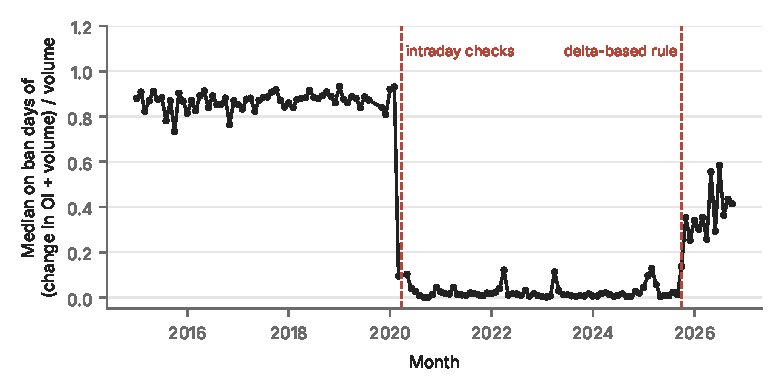
\includegraphics[width=0.75\textwidth]{fig_ban_R.pdf}
\caption{Monthly median of $(\Delta OI+V)/V$ on ban days (near and next futures, expiry days excluded).}\label{fig:R}
\end{figure}

\section{Does correction become one-sided? (H7)}
I regress the daily change in the basis on yesterday's deviation from the stock's median, separately in an upper regime
(above the stock's 80th percentile on non-ban days), a middle and a lower regime (below the 20th percentile), and let each
slope change on ban days. The model predicts that upward deviations revert more slowly in a ban ($\delta_{up}>0$) and
downward deviations as fast or faster.
\begin{table}[h]\centering\small
\caption{Reversion of the basis by regime, and its change in a ban}\label{tab:h7}
\begin{tabular}{lcc}
\toprule
& Normal slope (s.e.) & Change in a ban (s.e.) \\
\midrule
Upper regime & $-0.712$ (0.010) & $-0.089$ (0.037) \\
Middle & $-0.393$ (0.026) & $+0.099$ (0.062) \\
Lower regime & $-0.204$ (0.010) & $+0.081$ (0.030) \\
\bottomrule
\end{tabular}
\end{table}
The prediction fails, with the opposite sign: in a ban rich futures revert faster and cheap futures more slowly
(Table~\ref{tab:h7}). This holds with other threshold definitions, without imputed ban days and with the relative implied
repo rate; with the close-based basis the upper change is about zero. It is stronger on liquid days, differs by
enforcement period, and is concentrated in the first days of a spell ($-0.163$ in the first five calendar days against
$-0.008$ later). Instrumenting yesterday's deviation with the deviation two days earlier, to remove the effect of noise in
daily prices, gives $-0.190$ (s.e.\ 0.077) for the upper regime and $+0.088$ (0.015) for the lower: the result is not
caused by noisier prices on ban days.

A reading consistent with these facts, though not tested in advance, is that at the start of a ban the model's second
channel dominates: demand for new futures exposure is blocked, which removes the pressure that had made futures rich, so
upward deviations close quickly. The prediction tested was derived from the reduce-only arbitrage channel alone.

\section{The level of the basis when a ban starts}
\paragraph{Design.} Each ban spell from 2015 to September 2025 with no ban in the five days before it is an event. Controls
are other stocks in the same week with utilisation between 85\% and 95\% and no ban within five days, matched (up to five,
nearest by Mahalanobis distance) on the utilisation path of the previous five days and the basis on the day before. The
outcome is the change in the basis from the day before the ban, treated minus matched controls, averaged over the ban days
among the first five. Composition $C$ is the change in futures open interest over the five days before entry divided by
futures volume.

\paragraph{Results.} Over 889 matched entries the basis falls by 6.3\bp\ on average (median $-7.8$). With falling open
interest before entry ($C\le0$, 30 events) it rises by 8.4\bp\ (s.e.\ 10.9); with rising open interest it falls by 6.8\bp\
(s.e.\ 1.8). The difference, the pre-specified statistic, is $-15.2$\bp\ (one-sided $p=0.083$): the signs are those of the
model's level result, but the closing-pressure group is small because open interest must rise for utilisation to cross
95\%. Splitting at the median of $C$ instead gives a difference of $-5.8$ (s.e.\ 2.9, $p=0.025$), and $C$ as a continuous
variable gives $-4.8$ per standard deviation (s.e.\ 1.6, $p=0.001$). The basis returns to its earlier level about a week
after the start (Figure~\ref{fig:level}).

\begin{figure}[h]\centering
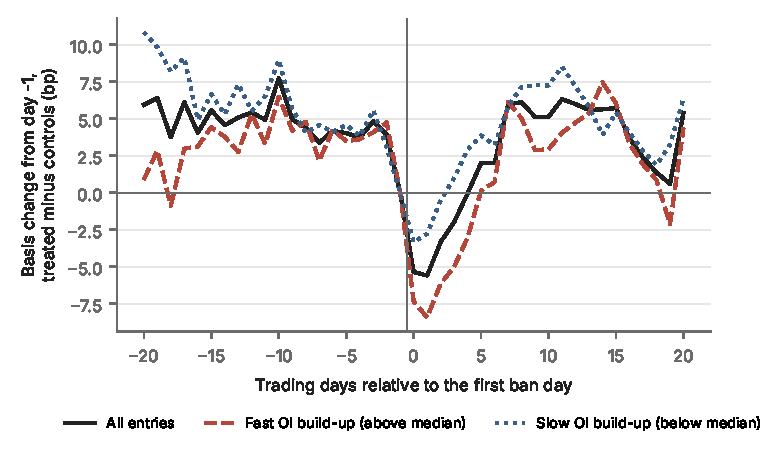
\includegraphics[width=0.8\textwidth]{fig_level_profile.pdf}
\caption{Change in the basis from the day before a ban starts, treated minus matched controls, by event time.}\label{fig:level}
\end{figure}

\paragraph{Caveats.} The matching leaves the treated basis 10\bp\ below that of the controls on the day before, and the
treated basis dips on that day; with the baseline taken over days $-10$ to $-2$, or controlling for the gap, the in-ban fall
is 9 to 11\bp\ and the composition slope stays negative. With controls from the same day only (685 events) the fall is
$-4.0$\bp\ (s.e.\ 2.0) but the composition gradient is not significant. Classifying events instead by the direction of
open interest and price (long build-up, short build-up, short covering, long unwinding), the in-ban fall appears for both
long build-up ($-7.9$\bp) and short build-up ($-5.5$\bp), so it is not specific to new long demand.

\section{The 95\% trigger}
\paragraph{Density.} Among stocks that were below 95\% the day before, the density of today's utilisation is smooth through
the trigger (Figure~\ref{fig:density}; Cattaneo, Jansson and Ma test, $T=-0.18$, $p=0.86$), across polynomial orders,
bandwidths and enforcement periods. Utilisation accelerates rather than stalls near the trigger: its mean daily change
is larger just below 95\%, and the share of stocks crossing the next day rises steadily to about one half at 0.93 to 0.95.
There is no sign that traders hold back to avoid a ban.

\begin{figure}[h]\centering
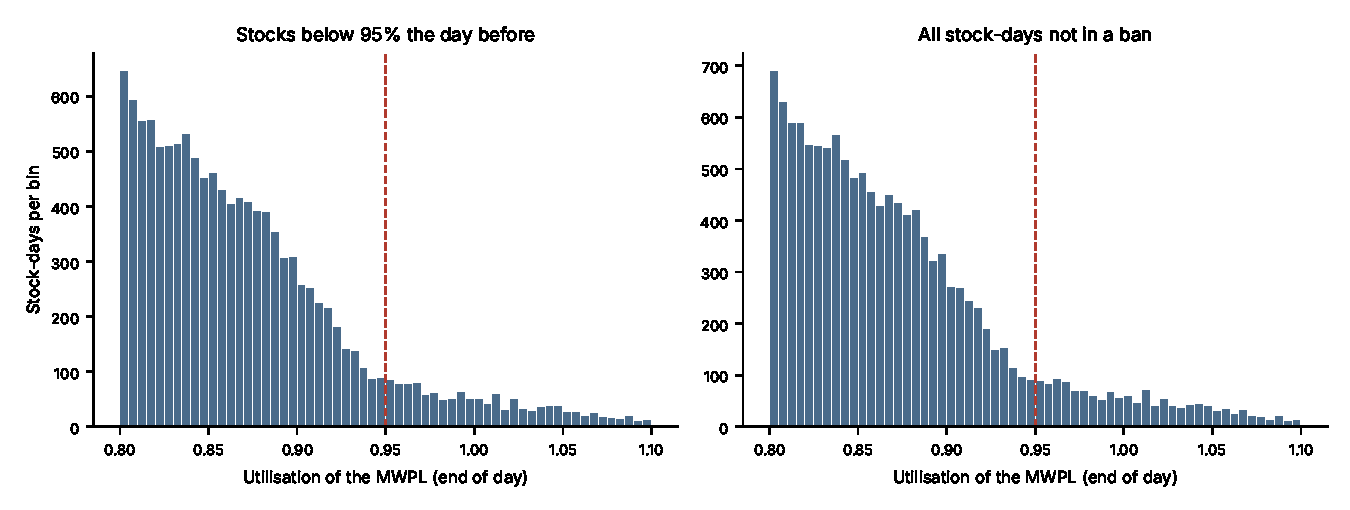
\includegraphics[width=0.85\textwidth]{density_95.pdf}
\caption{Utilisation at the end of the day. Left: stocks that were below 95\% the day before. Right: all stock-days not in
a ban (this population thins above 95\% by construction, because stocks above the trigger are in the ban the next day).}\label{fig:density}
\end{figure}

\paragraph{Regression discontinuity.} For stocks not in a ban the day before, crossing 95\% puts the stock in the ban the
next day in 99.7\% of cases. Local linear estimates with robust bias-corrected inference show sharp jumps in trading:
futures contracts $-1.53$ log points, $R$ $-0.66$, delivery share $+0.051$; cash volume does not jump. The basis level is
12.9\bp\ lower above the cutoff ($p=0.02$), but the basis is already 11.3\bp\ lower on the crossing day itself, before the ban
starts, and the change on the first ban day is small ($-2.8$, s.e.\ 4.1). The discontinuity therefore confirms the trading
mechanism but cannot separate a level effect of the ban from the pressure that pushes utilisation over the trigger.

\paragraph{Hysteresis.} Between 80\% and 95\% utilisation, stocks in a ban and stocks not in a ban can be compared at equal
utilisation. Controlling for utilisation, its change, five lags of the basis and stock and date fixed effects, being in a
ban changes the basis by $+0.4$\bp\ (s.e.\ 0.8, $p=0.64$); without the lags the difference is $-14.1$\bp. Banned stocks carry
the low basis of the start of the spell; the reduce-only state does not shift it further. Its effect on trading is as
strong as in H8.

\section{Bad news in a ban (H2)}
Of 8,586 results announcements of F\&O stocks, 179 fall on ban days, 55 of them bad news, so this test has little power, as
stated in advance. The drift after bad news is $-1.25\%$ outside bans relative to the middle tercile; in bans the additional
effect is $+0.7\%$ (s.e.\ 3.4). Outside bans the basis over the five days before an announcement is 2.0\bp\ lower before bad
news than before good news (s.e.\ 1.1, one-sided $p=0.04$), the pattern reported by Saurav, Srivastava and Agarwalla (2026);
inside bans the difference cannot be estimated with useful precision.

\section{Summary}
Bans bind hard on trading, and the identity that every trade closes positions holds once the rule is enforced on intraday
positions. The basis does not behave as the reduce-only arbitrage channel alone predicts: rich futures revert faster, and
the basis falls when a ban starts, more after fast build-ups of open interest. Both facts fit the model's second channel,
blocked new demand, but that reading was formed after seeing the results.
